\begin{frame}
    \frametitle{Transformaciones en 2D}
    \small
    \begin{center}
        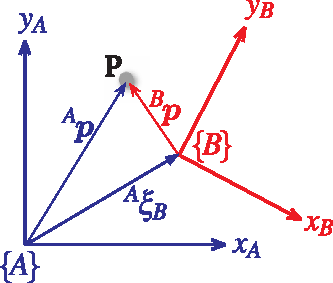
\includegraphics[width=0.3\columnwidth]{./images/coordinate_frames.pdf}
    \end{center}


    El punto $\point$ puede describirse mediante vectores de coordenadas relativos a cualquier marco $\{\mathrm{A}\}$ o $\{\mathrm{B}\}$. La pose de $\{\mathrm{B}\}$ relativa a $\{\mathrm{A}\}$ es $\transform{A}{B}$.
    \begin{align*}
        \pointCoord{A} &= \transform{A}{B}\pointCoord{B}\\
        \transform{A}{C} &= \transform{A}{B}\transform{B}{C}\\
        \transform{A}{B} &= \transform{B}{A}^{-1}
    \end{align*}

\end{frame}


\begin{frame}
    \frametitle{Transformaciones en 2D}
    
    \begin{figure}[!h]
        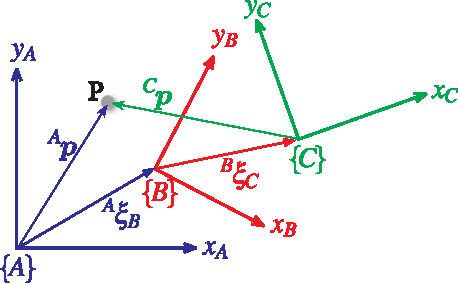
\includegraphics[width=0.6\columnwidth]{./images/multiple_coordinate_frames_2d.pdf}
    \end{figure}

\end{frame}


\begin{frame}
    \frametitle{Transformaciones en 3D}

    \begin{figure}[!h]
        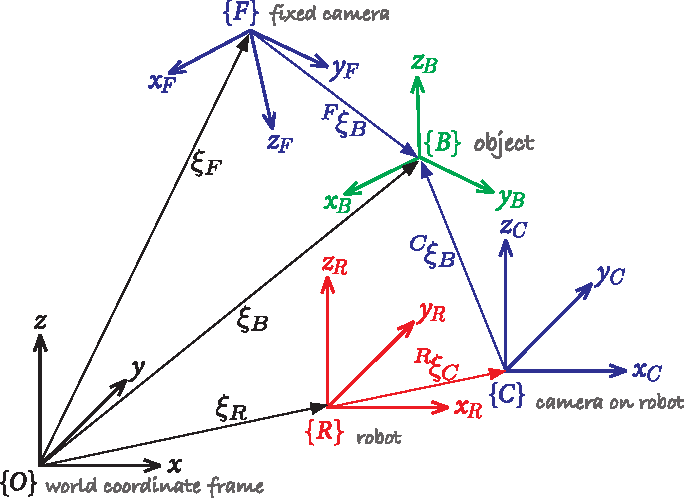
\includegraphics[width=0.6\columnwidth]{./images/multiple_coordinate_frames_3d.pdf}
    \end{figure}

\end{frame}

\begin{frame}
	\frametitle{Transformaciones...}
	
	\begin{figure}[!h]
		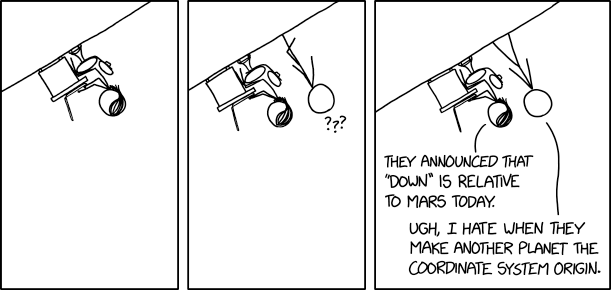
\includegraphics[width=\columnwidth]{./images/joke_coordinate_systems.png}
	\end{figure}
	
\end{frame}


\begin{frame}
    \frametitle{Rotación en 2D}

        \begin{center}
        \begin{minipage}{0.5\linewidth}
            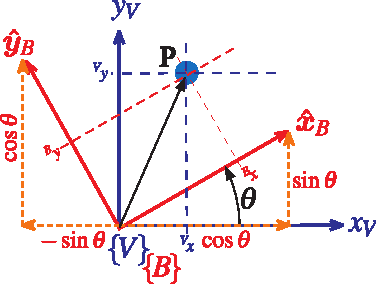
\includegraphics[width=\columnwidth]{coordinate_system_rotation.pdf}
        \end{minipage}
        \hspace{1em}
        \begin{minipage}{0.38\linewidth}
            \begin{equation*}
                {\displaystyle R(\theta )={\begin{bmatrix}\cos \theta &-\sin \theta \\\sin \theta &\cos \theta \\\end{bmatrix}}.}
            \end{equation*}

            \begin{equation*}
                {\displaystyle {\begin{bmatrix}x'\\y'\\\end{bmatrix}}={\begin{bmatrix}\cos \theta &-\sin \theta \\\sin \theta &\cos \theta \\\end{bmatrix}}{\begin{bmatrix}x\\y\\\end{bmatrix}}.}
            \end{equation*}

            \begin{equation*}
                \begin{aligned}x'&=x\cos \theta -y\sin \theta \,\\y'&=x\sin \theta +y\cos \theta \,\end{aligned}
            \end{equation*}

            \begin{equation*}
                \begin{bmatrix}
                    \toCoord{x}{V}\\
                    \toCoord{y}{V}
                \end{bmatrix} =
                \rotationCoord{V}{B}
                \begin{bmatrix}
                    \toCoord{x}{B}\\
                    \toCoord{y}{B}
                \end{bmatrix}
            \end{equation*}
        \end{minipage}
    \end{center}
\end{frame}


\begin{frame}
    \frametitle{Rototraslación en 2D}

    \begin{align*}
        \begin{bmatrix}
            \toCoord{x}{A}\\
            \toCoord{y}{A}
        \end{bmatrix} &=
        \begin{bmatrix}
            \toCoord{x}{B}\\
            \toCoord{y}{B}
        \end{bmatrix} +
        \begin{bmatrix}
            t_x\\
            t_y
        \end{bmatrix}\\
        \begin{bmatrix}
            \toCoord{x}{A}\\
            \toCoord{y}{A}
        \end{bmatrix} &=
        \begin{bmatrix}
            \cos \theta &-\sin \theta \\
            \sin \theta &\cos \theta \\
        \end{bmatrix}
        \begin{bmatrix}
            \toCoord{x}{B}\\
            \toCoord{y}{B}
        \end{bmatrix} +
        \begin{bmatrix}
            t_x\\
            t_y\\
        \end{bmatrix}
    \end{align*}

    \begin{equation*}
        \begin{bmatrix}
            \toCoord{x}{A}\\
            \toCoord{y}{A}\\
            1
        \end{bmatrix} =
        \begin{bmatrix}
            \rotationCoord{A}{B} & \translation\\
            \vec{0} & 1
        \end{bmatrix}
        \begin{bmatrix}
            \toCoord{x}{B}\\
            \toCoord{y}{B}\\
            1
        \end{bmatrix}
    \end{equation*}

    \begin{equation*}
        \begin{bmatrix}
            \toCoord{x}{A}\\
            \toCoord{y}{A}\\
        \end{bmatrix} = R(\theta )
        \begin{bmatrix}
            \toCoord{x}{B}\\
            \toCoord{y}{B}
       \end{bmatrix} + \translation
    \end{equation*}
\end{frame}


\begin{frame}
    \frametitle{Algunas Propiedades de las transformaciones}

	Composición:
    \begin{equation*}
        \transform{}{1}\transform{}{2} =
        \begin{bmatrix}
            \rotationCoord{}{1} & \translationCoord{}{1}\\
            \vec{0} & 1
        \end{bmatrix}
        \begin{bmatrix}
            \rotationCoord{}{2} & \translationCoord{}{2}\\
            \vec{0} & 1
        \end{bmatrix} =
        \begin{bmatrix}
            \rotationCoord{}{1}\rotationCoord{}{2} & \translationCoord{}{1}+\rotationCoord{}{1}\translationCoord{}{2}\\
            \vec{0} & 1
        \end{bmatrix}
    \end{equation*}

	Inversa:
    \begin{equation*}
        \transform{}{}^{-1}=
        \begin{bmatrix}
            \rotation & \translation\\
            \vec{0} & 1
        \end{bmatrix}^{-1} =
        \begin{bmatrix}
            \rotation^{\top} & -\rotation^{\top}\translation\\
            \vec{0} & 1
        \end{bmatrix}
    \end{equation*}

\end{frame}


\begin{frame}
	\frametitle{Pose}
	
	La Pose (posición y orientación) de un robot es la transformación rototraslacional dada por la posición y orientación del robot en el espacio.
	
	Ejemplo: Dado el vector posición $\position$ y la matriz orientación $\orientation$ del robot $\bodyCoordSystem$ en el mundo $\worldCoordSystem$, notamos la pose como $\transform{\worldCoordSystem}{\bodyCoordSystem}$
	
	\begin{equation*}
		\transform{\worldCoordSystem}{\bodyCoordSystem}=
		\begin{bmatrix}
			\orientation & \position\\
			\vec{0} & 1
		\end{bmatrix}
	\end{equation*}

	Observar que la pose es una transformación que toma elementos en coordenadas del robot y los devuelve en coordenadas del mundo.
\end{frame}


\begin{frame}
    \frametitle{Coordenadas Homogeneas e Hinomogeneas}
    Un vector $\point = (x, y)$ se escribe en forma homogénea como $\homo{\point} \in P^2$, $\homo{\point} = (x1, x2, x3)$ donde $x = \dfrac{x_1}{x_3}$, $y= \dfrac{x_2}{x_3}$ y $x_3 \neq 0$. La dimensión se ha incrementado en uno y un punto en un plano ahora está representado por un 3-vector. Para convertir un punto a una forma homogénea, normalmente agregamos un elemento igual a uno $\homo{\point} = (x, y, 1)$. La tilde indica que el vector es homogéneo.


    Los vectores homogéneos tienen la propiedad importante de que $\homo{\point}$ es equivalente a $\lambda \homo{\point}$ para todo $\lambda \neq 0$ que escribimos como $\homo{\point} = \lambda \homo{\point}$. Es decir, $\homo{\point}$ representa el mismo punto en el plano independientemente del factor de escala general.
\end{frame}

\begin{frame}
    \frametitle{Rotación en 3D}
    \small
    \begin{equation*}
        {\displaystyle {\begin{alignedat}{1}R_{x}(\theta )&={\begin{bmatrix}1&0&0\\0&\cos \theta &-\sin \theta \\[3pt]0&\sin \theta     &\cos \theta \\[3pt]\end{bmatrix}}\\
                    R_{y}(\theta )&={\begin{bmatrix}\cos \theta &0&\sin \theta \\[3pt]0&1&0\\[3pt]-\sin \theta &0&\cos \theta \\
                    \end{bmatrix}}\\
                    R_{z}(\theta )&={\begin{bmatrix}\cos \theta &-\sin \theta &0\\[3pt]\sin \theta &\cos \theta &0\\[3pt]0&0&1\\\end{bmatrix}}\end{alignedat}}
        }
    \end{equation*}

    Ejemplo:
    \begin{equation*}
        {\displaystyle R_{z}(90^{\circ }){\begin{bmatrix}1\\0\\0\\\end{bmatrix}}={\begin{bmatrix}\cos 90^{\circ }&-\sin 90^{\circ }&0\\\sin 90^{\circ }&\quad \cos 90^{\circ }&0\\0&0&1\\\end{bmatrix}}{\begin{bmatrix}1\\0\\0\\\end{bmatrix}}={\begin{bmatrix}0&-1&0\\1&0&0\\0&0&1\\\end{bmatrix}}{\begin{bmatrix}1\\0\\0\\\end{bmatrix}}={\begin{bmatrix}0\\1\\0\\\end{bmatrix}}}
    \end{equation*}

\end{frame}

\begin{frame}
	\frametitle{Rotaciones Generales 3D: Rotaciones Extrínsecas vs Rotaciones Intrínsecas}

	\begin{block}{Rotación Intrínseca}
	Describe una rotación en relación con el sistema de coordenadas local del objeto. Los ejes del objeto pueden cambiar durante la rotación.
	\end{block}

    \begin{center}
        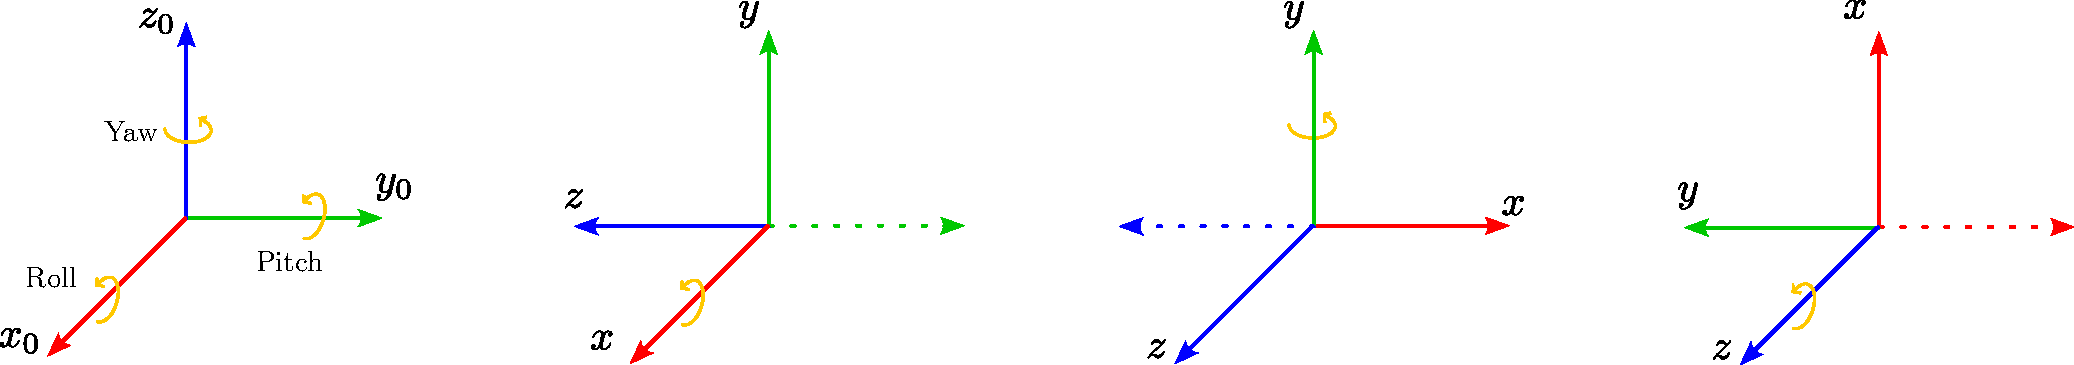
\includegraphics[width=0.7\columnwidth]{./images/intrinsic_rotation.pdf}
    \end{center}

	\begin{block}{Rotación Extrínseca}
		Describe una rotación en relación con un sistema de coordenadas global fijo en el espacio. El sistema de referencia es externo al objeto que está siendo rotado.
	\end{block}
	
    \begin{center}
        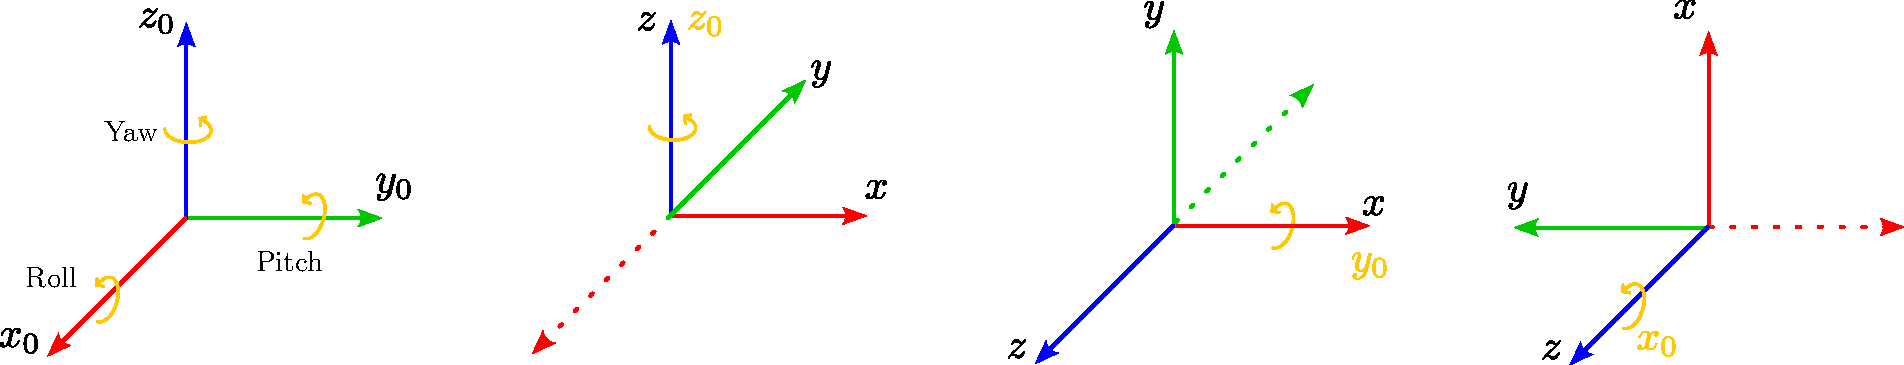
\includegraphics[width=0.7\columnwidth]{./images/extrinsic_rotation.pdf}
    \end{center}
		
	
	\note{Copiar slides donde se muestra que las rotaciones intrínsecas son equivalentes a las rotaciones extrínsecas: https://www.youtube.com/watch?v=icczqt73B7o}
	
\end{frame}

\begin{frame}
    \frametitle{Rotaciones generales 3D}
    \tiny
    
    Rotación intrínseca con ángulos yaw, pitch y roll como $\alpha$, $\beta$ y $\gamma$. Formalmente, es una rotación intrínseca con ángulos Tait–Bryan angles $\alpha$, $\beta$ y $\gamma$ sobre los ejes $z$, $y$, $x$.
    \begin{equation*}
        {\displaystyle
            {
                \begin{aligned}
                    R=R_{z}(\alpha )\,R_{y}(\beta )\,R_{x}(\gamma )&={\overset {\text{yaw}}{\begin{bmatrix}\cos \alpha &-\sin \alpha &0\\\sin \alpha &\cos \alpha &0\\0&0&1\\\end{bmatrix}}}{\overset {\text{pitch}}{\begin{bmatrix}\cos \beta &0&\sin \beta \\0&1&0\\-\sin \beta &0&\cos \beta \\\end{bmatrix}}}{\overset {\text{roll}}{\begin{bmatrix}1&0&0\\0&\cos \gamma &-\sin \gamma \\0&\sin \gamma &\cos \gamma \\\end{bmatrix}}}\\
                    &={\begin{bmatrix}\cos \alpha \cos \beta &\cos \alpha \sin \beta \sin \gamma -\sin \alpha \cos \gamma &\cos \alpha \sin \beta \cos \gamma +\sin \alpha \sin \gamma \\\sin \alpha \cos \beta &\sin \alpha \sin \beta \sin \gamma +\cos \alpha \cos \gamma &\sin \alpha \sin \beta \cos \gamma -\cos \alpha \sin \gamma \\-\sin \beta &\cos \beta \sin \gamma &\cos \beta \cos \gamma \\\end{bmatrix}
                    }
                \end{aligned}
            }
        }
    \end{equation*}
    De manera similar rotación extínseca con ángulos de Euler $\alpha$, $\beta$ y $\gamma$ sobre los ejes $x$, $y$ y $z$.
    \begin{equation*}
        {\displaystyle \begin{aligned}
                R=R_{z}(\gamma )\,R_{y}(\beta )\,R_{x}(\alpha )&={\begin{bmatrix}\cos \gamma &-\sin \gamma &0\\\sin \gamma &\cos \gamma &0\\0&0&1\\\end{bmatrix}}{\begin{bmatrix}\cos \beta &0&\sin \beta \\0&1&0\\-\sin \beta &0&\cos \beta \\\end{bmatrix}}{\begin{bmatrix}1&0&0\\0&\cos \alpha &-\sin \alpha \\0&\sin \alpha &\cos \alpha \\\end{bmatrix}}\\
                &={\begin{bmatrix}
                        \cos \beta \cos \gamma & \sin \alpha \sin \beta \cos \gamma - \cos \alpha \sin \gamma & \cos \alpha \sin \beta \cos \gamma + \sin \alpha \sin \gamma \\
                        \cos \beta \sin \gamma & \sin \alpha \sin \beta \sin \gamma + \cos \alpha \cos \gamma & \cos \alpha \sin \beta \sin \gamma - \sin \alpha \cos \gamma \\
                        -\sin \beta & \sin \alpha \cos \beta & \cos \alpha \cos \beta \\
                \end{bmatrix}}
            \end{aligned}
        }
    \end{equation*}

\note{Davenport demostró que se puede lograr descomponer cualquier orientación mediante la sucesión de tres rotaciones elementales utilizando ejes no ortogonales. Las rotaciones elementales pueden darse respecto a los ejes del sistema de coordenadas fijo (rotaciones extrínsecas) o sobre los ejes de un sistema de coordenadas giratorio, que inicialmente se alinea con el sistema de ejes fijo y modifica su orientación después de cada rotación elemental (rotaciones intrínsecas).

Según el teorema de Davenport, es posible una descomposición única si y solo si el segundo eje es perpendicular a los otros dos ejes. Por lo tanto, los ejes 1 y 3 deben estar en el plano ortogonal al eje 2.

En consecuencia, las descomposiciones de las rotaciones encadenadas de Euler y de las rotaciones encadenadas de Tait-Bryan son casos particulares de esta configuración general. El caso de Tait-Bryan aparece cuando los ejes 1 y 3 son perpendiculares, y el caso de Euler aparece cuando se superponen.
}

\end{frame}


\begin{frame}
	\frametitle{Rotaciones generales 3D}

	
	Una rotación de un marco de referencia a otro se puede obtener mediante la multiplicación de varias rotaciones.
	
	Rotación Intrínseca
	$R = R_{x} R_{y} R_{z}$
	
	
	\TODO{SLIDE a realizar...}
	
	$x-y\prime-z\prime\prime$ (intrinsic rotations) or $z-y-x$ (extrinsic rotations)\\
	$y-z\prime-x\prime\prime$ (intrinsic rotations) or $x-z-y$ (extrinsic rotations)\\
	$z-x\prime-y\prime\prime$ (intrinsic rotations) or $y-x-z$ (extrinsic rotations)\\
	$x-\prime-y\prime\prime$ (intrinsic rotations) or $y-z-x$ (extrinsic rotations)\\
	$z-y\prime-x\prime\prime$ (intrinsic rotations) or $x-y-z$ (extrinsic rotations): the intrinsic rotations are known as: yaw, pitch and roll\\
	$y-x\prime-\prime\prime$ (intrinsic rotations) or $z-x-y$ (extrinsic rotations)\\
	
	
	\note{Copiar slides donde se muestra que las rotaciones intrínsecas son equivalentes a las rotaciones extrínsecas: https://www.youtube.com/watch?v=icczqt73B7o}
	
\end{frame}


\begin{frame}
    \frametitle{Propiedades de matrices Rotación}
    \small
    \begin{itemize}
        \item $R^{\mathsf {T}}=R^{-1}$ Matriz ortogonal
        \item $\det R = \pm 1$ (esto implica que la longitud del vector no cambia luego de la rotación)
        \item $R \in SO(3)$ entonces $\rotationCoord{A}{C} = \rotationCoord{A}{B} \rotationCoord{B}{C}$ y $\rotationCoord{A}{B} = \rotationCoord{B}{A}^{-1}$
    \end{itemize}

    Determinar el ángulo de una matriz de rotación utilizando la traza de la matriz (la suma de los elementos de la diagonal del matriz).
    \begin{equation*}
        {\displaystyle \operatorname {tr} (R)=1+2\cos \theta ,}
    \end{equation*}

    \begin{equation*}
        {\displaystyle |\theta |=\arccos \left({\frac {\operatorname {tr} (R)-1}{2}}\right).}
    \end{equation*}

\end{frame}

\begin{frame}
    \frametitle{Rotación representada con Axis-angle}
    La notación axial-angular es equivalente al más conciso vector de rotación, también llamado vector de Euler. En este caso, tanto el eje de rotación como el ángulo están representados por un vector codireccional con el eje de rotación cuyo módulo (longitud) coincide con el ángulo de rotación $\theta$,
    \begin{center}
        \begin{minipage}{0.38\linewidth}
            \small
            \begin{equation*}
                {\displaystyle {\boldsymbol {\theta }}=\theta \mathbf {e} \,.}
            \end{equation*}
            \begin{equation*}
                {\displaystyle (\mathrm {eje} ,\mathrm {\text{ángulo}} )=\left({\begin{bmatrix}e_{x}\\e_{y}\\e_{z}\end{bmatrix}},\theta \right)}
            \end{equation*}
        \end{minipage}
        \hspace{1em}
        \begin{minipage}{0.38\linewidth}
            \centering
            \begin{figure}
	           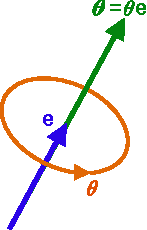
\includegraphics[width=0.3\columnwidth]{images/axis_angle_vector.pdf}
            \end{figure}
        \end{minipage}
    \end{center}

    Ejemplo un vector de rotación con una magnitud de $\dfrac{\pi}{2}$ apuntando en la dirección $z$:
    \begin{equation*}
        {\displaystyle {\left({\begin{bmatrix}0\\0\\1\end{bmatrix}},{\frac {\pi }{2}}\right) = \begin{bmatrix}0\\0\\{\frac {\pi }{2}}\end{bmatrix}}.}
    \end{equation*}

    \note{The representation is very intuitive, but for actually applying the rotation, another representation is required, such as a quaternion or rotation matrix.}

\end{frame}

\begin{frame}
    \frametitle{Quaternions}
    Los cuaterniones es una generalización de números complejos con tres números imaginarios (i, j y k). Es un número complejo de cuatro dimensiones que se puede utilizar para representar la orientación de un cuerpo rígido o un marco de coordenadas en un espacio tridimensional. La definición general de un cuaternión viene dada por:
    %
    \begin{equation*}
        q = w + q_x i + q_y j + q_z k = \begin{bmatrix} q_w & q_x & q_y & q_z\end{bmatrix}
    \end{equation*}
\end{frame}

\begin{frame}
    \frametitle{Quaternions}

    \begin{center}
        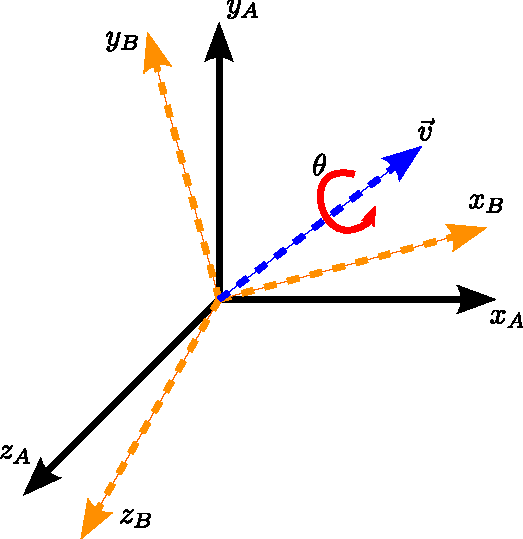
\includegraphics[width=0.2\columnwidth]{./images/quaternion.pdf}
    \end{center}

    Los cuaterniones representan una transformación de rotación en 3D. Por lo tanto, la forma más fácil de representar un cuaternión es imaginar la rotación de un ángulo dado alrededor de un vector dado. La figura ilustra la rotación del ángulo $\theta$ alrededor del vector $\vec{v} = [v_{x} v_{y} v_{z}]$. El cuaternión asociado a esta rotación está dado por:
    %
    \begin{align*}
        q &= \begin{bmatrix} q_w & q_x & q_y & q_z\end{bmatrix}\\
        q &= \begin{bmatrix}
            \cos \frac{\theta}{2} & v_{x} \sin \frac{\theta}{2} & v_{y} \sin \frac{\theta}{2} & v_{z}\sin \frac{\theta}{2}
        \end{bmatrix}
    \end{align*}
\end{frame}

\begin{frame}
    \frametitle{Right-hand rule}
    En Robótica la disposición de los ejes de coordenadas y el sentido de rotación de los mismos está dado por la regla de la mano derecha (Right-hand rule).

    \begin{figure}[!h]
        \centering
        \subfloat[]
        {
            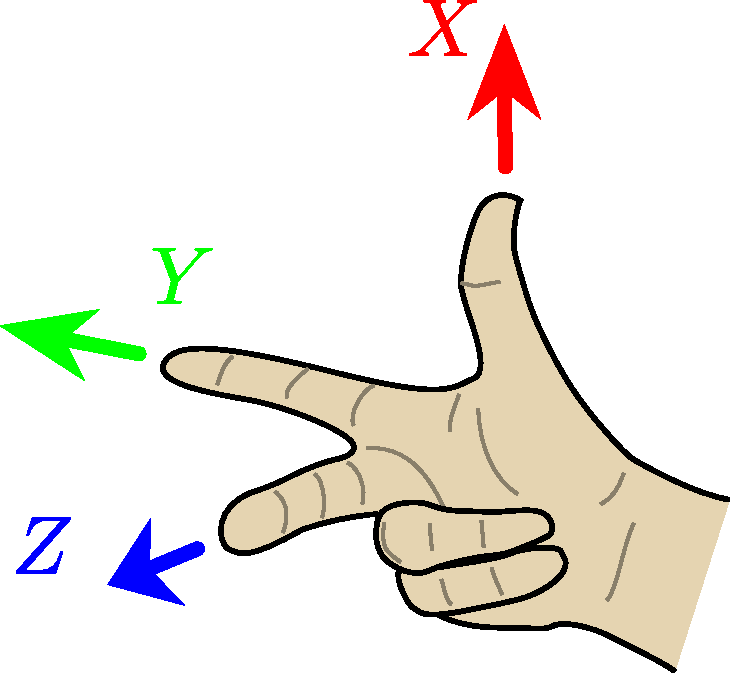
\includegraphics[width=0.4\columnwidth]{./images/right_hand_rule.pdf}
        }\hspace{1cm}
        \subfloat[]
        {
            
\includegraphics[width=0.4\columnwidth]{./images/right_hand_rule_positive_rotation.pdf}
        }
    \end{figure}
\end{frame}

\begin{frame}
    \frametitle{Roll Pitch Yaw }
    
    \begin{figure}[!h]
        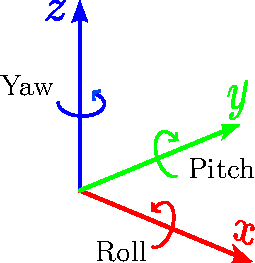
\includegraphics[width=0.4\columnwidth]{./images/roll_pitch_yaw.pdf}
    \end{figure}
    \TODO{Gimbal-Lock Video explanation: https://youtu.be/-WXfEPg8eMM}
\end{frame}

\begin{frame}
    \frametitle{Left-hand vs Right-hand rule}

        \only<1>{
        	    \begin{figure}
        	    	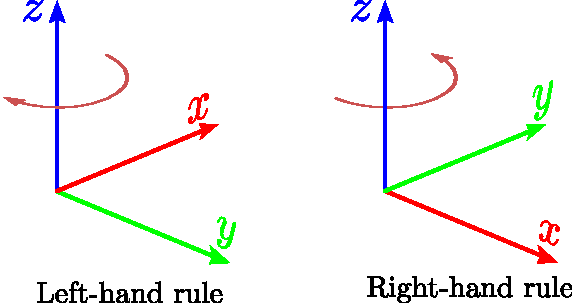
\includegraphics[width=0.9\columnwidth]{./images/left_right_hand_rule.pdf}
	    	    \end{figure}
            	}
        \only<2>{
        	\begin{figure}
    	    	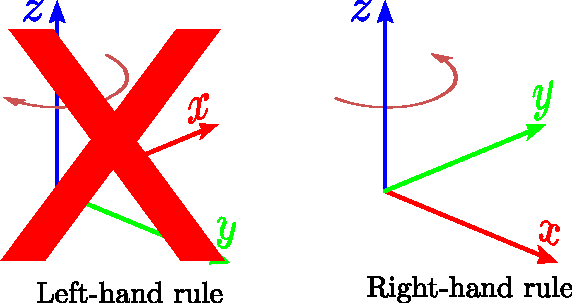
\includegraphics[width=0.9\columnwidth]{./images/left_right_hand_rule_cross.pdf}
	        \end{figure}
        }
\end{frame}

